\documentclass{article} % Replace with neurips template as required
\usepackage[utf8]{inputenc}
\usepackage{graphicx}
\usepackage{booktabs}
\usepackage{amsmath}
\usepackage{hyperref}

\title{Analyzing Catastrophic Forgetting in MLPs on Permuted-MNIST}
\author{Pavan Prasad Gorintla}
\date{CS 599: Foundations of Deep Learning --- Lab 2}

\begin{document}
\maketitle

\section{Problem and Setup}
We follow the lab brief to study catastrophic forgetting using Permuted-MNIST with $T{=}10$ tasks, a standard MLP with depths $\{2,3,4\}$ (256 hidden units), and a sequential training schedule of $50 + 9\times 20 = 230$ epochs.
We report the Resulting Task Matrix $R$ and compute ACC and BWT exactly as defined in the instructions.

\section{Methods}
\textbf{Model:} MLP with ReLU activations, optional dropout $\leq 0.5$, and softmax output (10 classes).\\
\textbf{Loss:} Negative log-likelihood (sparse cross entropy) with optional L1/L2/L1+L2 kernel regularization.\\
\textbf{Optimizers:} SGD, Adam, RMSprop.\\
\textbf{Data:} For each task $t$, a fixed random pixel permutation is applied to MNIST.

\section{Metrics}
ACC $= \frac{1}{T}\sum_{i=1}^{T} R_{T,i}$,\quad
BWT $= \frac{1}{T-1}\sum_{i=1}^{T-1} (R_{T,i} - R_{i,i})$.\\
We also report TBWT and CBWT (bonus).

\section{Results (Fill from outputs)}
Table~\ref{tab:depth} shows depth ablation with dropout and optimizer fixed.
Replace placeholders with values from \texttt{metrics.json}.

\begin{table}[h]
\centering
\begin{tabular}{lcccc}
\toprule
Setting & ACC & BWT & TBWT & CBWT \\
\midrule
Depth=2, loss=NLL, opt=SGD & \_\_\_ & \_\_\_ & \_\_\_ & \_\_\_ \\
Depth=3, loss=NLL, opt=SGD & \_\_\_ & \_\_\_ & \_\_\_ & \_\_\_ \\
Depth=4, loss=NLL, opt=SGD & \_\_\_ & \_\_\_ & \_\_\_ & \_\_\_ \\
\bottomrule
\end{tabular}
\caption{Depth ablation summary.}
\label{tab:depth}
\end{table}

\begin{figure}[h]
\centering
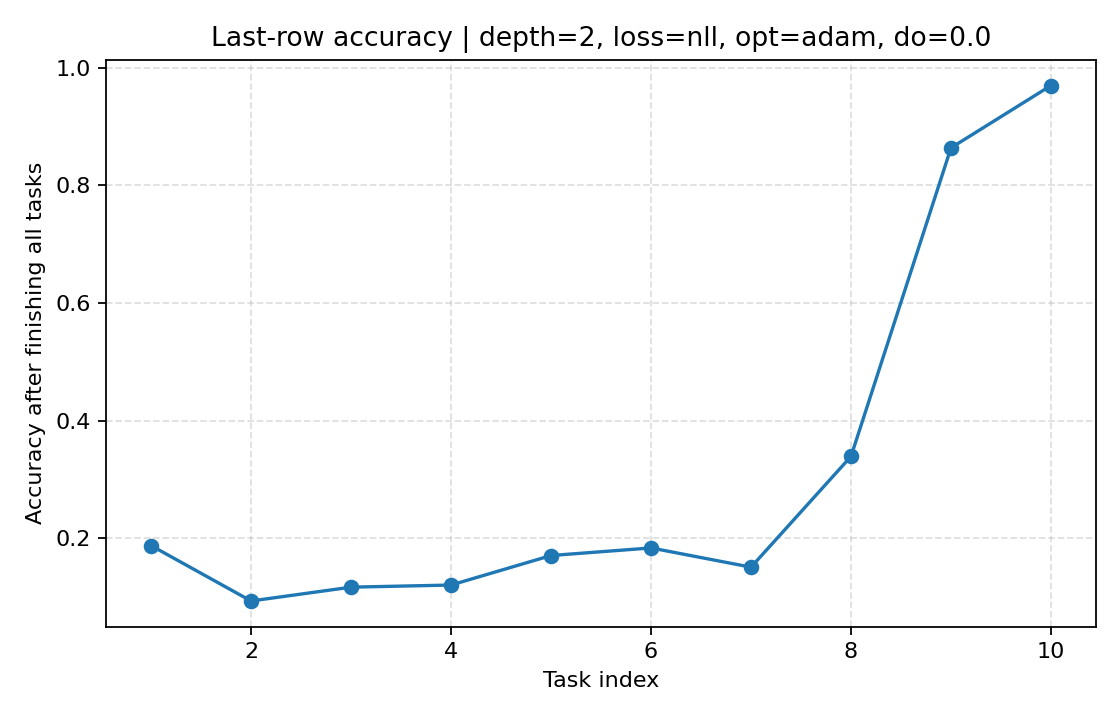
\includegraphics[width=0.72\linewidth]{last_row.png}
\caption{Accuracy by task after finishing all tasks (example run).}
\end{figure}

\section{Discussion}
Summarize: effect of depth, dropout, optimizer, and L1/L2 on forgetting; trends visible in $R$; which choices reduce negative BWT; limitations and future work (e.g., EWC, replay).

\section{References}
Cite the lab brief and continual-learning papers as required.
\end{document}
